\documentclass[10pt,a4paper]{article}
\usepackage[utf8]{inputenc}
\usepackage{amsmath}
\usepackage{amsfonts}
\usepackage{amssymb}
\usepackage{enumitem}
\usepackage{graphicx}
\usepackage{ulem}
\usepackage{enumitem}
\usepackage[official]{eurosym}
\title{Advanced Databases \& noSQL (INFDEV03-5) \\ Assignment 3}
\author { }
\date { }
\begin{document}
\maketitle

\section*{Instructions}
\begin{itemize}[noitemsep]
\item The assignment must be implemented using Neo4j.
\item Deliver the cypher queries into a \underline{text} file (not word!).
\item Deliver also the database folder of Neo4j (your \texttt{database\textunderscore name.graphdb}).
\end{itemize}

\textbf{You can do either assignment A or B}

\section*{Assignment A}
Consider the Entity-Relationship diagram in Figure \ref{fig:erd} representing the model for an airport database.

\begin{itemize}[noitemsep]
	\item Give a graph database implementation in Neo4j. Fill in the database with data satisfying the following constraints:
		\begin{itemize}
			\item At least 6 airports, two of which must be name 'Schiphol', and 'Venezia Marco Polo', two must be located in 'London', and one in 'Rome'.
			\item The values of \texttt{size} in \texttt{airports} must be 'Small', 'Medium', or 'Large'.
			\item At least one airport must be 'Large'.
			\item Each airport must have at least 5 terminals.
			\item 'Venezia Marco Polo' must have a terminal 'B'.
			\item At least 5 companies, two of which must be 'Lufthansa' and 'KLM'.
			\item At least 5 flights, one of which must be scheduled before 15:00.
			\item At least 3 gates per terminal.
			\item The values for \texttt{state} in \texttt{gates} must be either 'Boarding' or 'Closed'.
			\item There must be a 'Boarding' gate for terminal 'B' in 'Venezia Marco Polo'.
		\end{itemize}
	\item Implement the following queries in cypher:
		\begin{enumerate}[noitemsep]
			\item Find the name and the capacity of all 'Large' airports.
			\item Find the total capacity of the airports in the same city. Output the name of the city and the total capacity.
			\item Find the name of the airport with the highest capacity. Output the name and the capacity.
			\item Find all the opened terminals in 'Schiphol'. Output the code.
			\item Find all the terminals of the airports in 'London'. Output the code.
			\item Find all the gates that are boarding in 'Venezia Marco Polo' for terminal 'B'. Print the number and the state.
			\item Find all the flights landing in 'Rome' for 'Lufthansa' and 'KLM'. Print the code and the plane.
			\item For each company find the amount of flights going to 'Rome' leaving before 15:00. Print the company name and the total of flights.
		\end{enumerate}
\end{itemize}

\begin{figure}
	\centering
	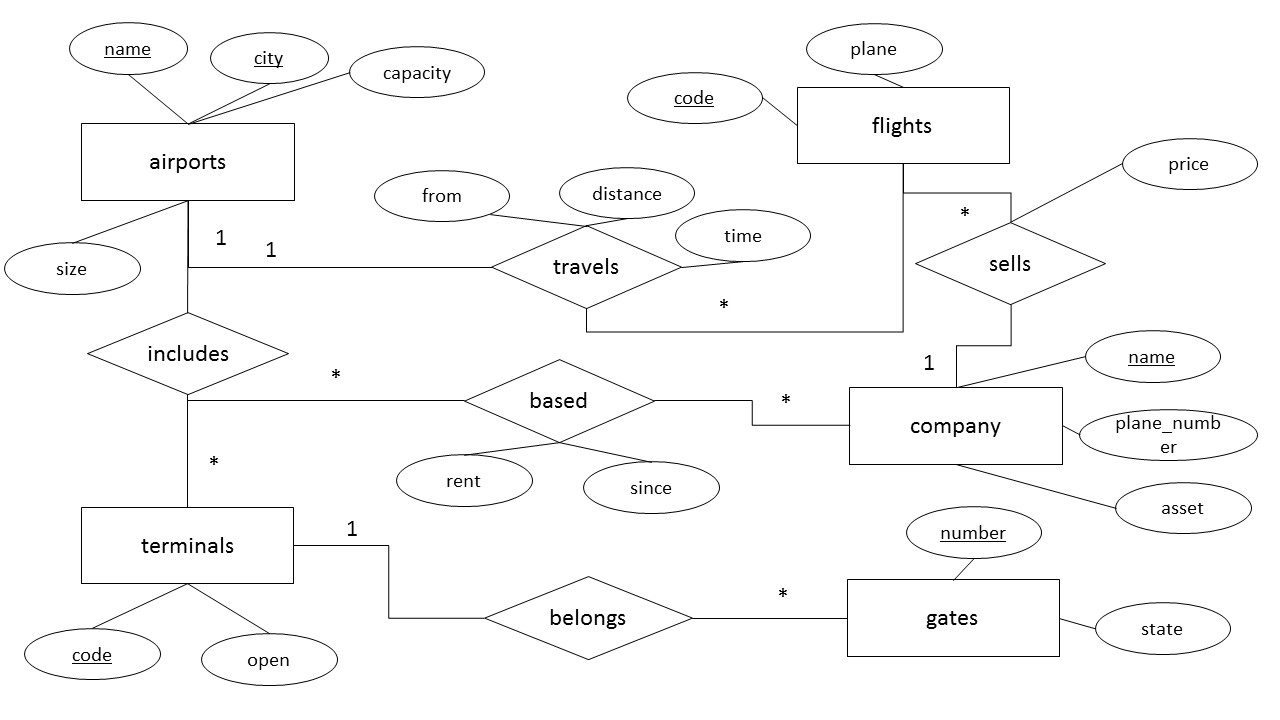
\includegraphics[scale = 0.42]{img/erd_assignment3}
	\caption{ER Diagram for the assignment}
	\label{fig:erd}
\end{figure}

\section*{Assignment B}

Consider the normalized table structure you have created for assignment 1 about the multinational company application. Your tasks are:
\begin{itemize}
\item  	Re-factor the application in order to use it with the graph database (Neo4j)
\item 	Re-implement the CRUD operations for each table to get work with the graph database
\item  	Map 5 entity sets and their relationships from your relational database to the equivalent structure in graph database 
\item Reimplement the queries from assignment 2 using cypher queries and show the results in your application
\begin{enumerate}
	\item An employee is underworking if he is working less than 5 hours on his projects, he is working normally if he is working between 5 and 20 hours, and he is overworking if he is working more than 20 hours. Output the number of employees that are overworking per project.
	\item Find the total working hours of all employees and average working hours per employee.
	\item Find the total fee of an employee. This number is obtained by multiplying the working hours on all the projects by the hour fee of his position.
\end{enumerate}
\end{itemize}


\end{document}